\documentclass{beamer}
\usepackage{beamerthemeshadow}
\usepackage{color}
\usepackage{graphicx}

\mode<presentation>
{
  \usetheme{Warsaw} %%% Change later
 \usecolortheme{dove}


  \setbeamercovered{invisible}
  % or whatever (possibly just delete it)
}
\setbeamertemplate{footline}[page number]{}


\begin{document}
\title{Adapting Clojure to an introductory CS classroom.}
\author{Elena Machkasova}
\institute[UMM] % (optional, but mostly needed)
{
 % \inst{1}%
  University of Minnesota, Morris
}
\date[]  
{Clojure/west, April 21 2015.}

\begin{frame}
  \titlepage
\end{frame}

\section{Why Clojure for intro CS?}

\begin{frame}
   \frametitle{ClojurEd project}
ClojurEd is a project at UMM: developing a beginner-friendly setup for Clojure. 
\uncover<2>{
\begin{figure}
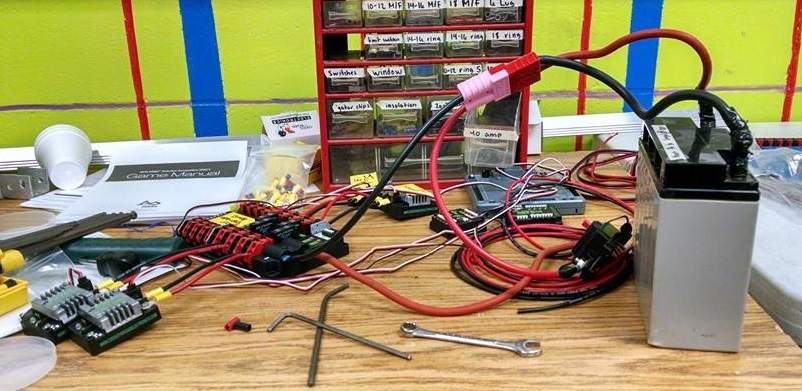
\includegraphics[scale=0.4]{work-in-progress.jpg}
\end{figure}
This is work in progress!

{\large\bf  Lots}  still needs to be done before we can use Clojure in an introductory class. 
}
\end{frame}

\begin{frame}
   \frametitle{Where are we coming from?}
\begin{figure}
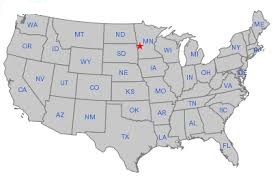
\includegraphics[scale=0.7]{morris.jpg}
\end{figure}
%{\tt Need a map here; need to make bullet points appear one by one}
\begin{itemize}
\item Morris: rural town 3.5 hours from UMN-TC. 
\item UMM:  small undergraduate-only liberal arts college.
\item Undergraduate research. 
\item<2>Use Lisp in an introductory CS class. 
\end{itemize}
\end{frame}

\begin{frame}
   \frametitle{A programming language for introductory class}
\begin{itemize}
\item {\bf Use} a programming language in an introductory class.
\item <2->{\bf  Teach} concepts and skills.
\item <3-> {\bf  Teach} CS-style problem solving.
\item <4->The language needs to be simple, well-defined, and non-distracting (Felleisen et al, 2004).
\item <5->Dynamically typed.
\item <6-> Functional languages offer focus on functions, modularity, abstraction.
\item <7-> Understanding of higher order functions may be useful later for parallel programming and Javascript-based web dev. 
\item <8-> Interactive development promotes testing: REPL. 
%\item Lisps have simple syntax and clearly defined semantics.
\end{itemize}
\end{frame}

\begin{frame}
   \frametitle{Current use of Lisp/Clojure in classes}
\begin{itemize}
\item UMM uses Racket (a Lisp) in an introductory class. 
\item 2010: a UMM student mentioned Clojure. 
\item We've used Clojure in upper-level courses (Programming Languages, Programming for Parallel Architecture).
%\item Would like to use it in an introductory class (it's a long way).
%\item Other schools using Clojure: Hampshire College, MA, maybe more? 
\end{itemize}
\end{frame}

\begin{frame}
   \frametitle{What Clojure brings to the table?}
Students are curious, would like to expand and apply what they learn. 

Clojure offers:
\begin{itemize}
\item A large community that students can explore/benefit from: libraries, community-maintained docs, textbooks, blog posts, open source projects, meetups,....
\item Concurrency.
\item Integration with Java. 
\item Elena's subjective opinion: collections done right. 
\end{itemize}
\end{frame}

\section{Why {\bf not} (yet) Clojure}

\begin{frame}
   \frametitle{What's lacking}
\begin{itemize}
\item Usability of error messages. %{\tt give an example}
\item Beginner-friendly IDE. 
\item Beginner-friendly project manager. 
%\item Can't expect new students use emacs/vim and command line (at least if we want to keep CS enrollments/diversity). 
\item Beginner-friendly graphical libraries. 
\item More uniform (from a beginner's standpoint) behavior of strings, collections vs sequences, etc.  
\item Beginner-friendly textbooks (focus on concepts, use language as a learning tool). 
\end{itemize}
\end{frame}

\section{Error messages transformations}
\begin{frame}[fragile]
   \frametitle{(Non)Usability of error messages}
\begin{verbatim}
Exception in thread "main" java.lang.RuntimeException:
EOF while reading, starting at line 3,
compiling:(student/example.clj:4:1)
	at clojure.lang.Compiler.load(Compiler.java:7137)
	at clojure.lang.RT.loadResourceScript(RT.java:370)
	at clojure.lang.RT.loadResourceScript(RT.java:361)....
\end{verbatim}
\begin{itemize}
\item Phrased in terms of Java types and unfamiliar terminology.
\item Java stack trace. 
\item Often misleading. 
\item Not well integrated with IDEs (LightTable does some line highlighting). 
\item Come from compiler, run-time system, REPL, testing frameworks %(makes integration with IDE difficult). 
\end{itemize}
\end{frame}

\begin{frame}[fragile]
   \frametitle { What do we do about error messages}
\begin{itemize}
\item Our message:
\begin{verbatim}
Compilation error: end of file, starting at line 3,
while compiling student/example.clj.
Probably a non-closing parenthesis or bracket.
\end{verbatim}
\item Filter stack trace. 
\item Transform using regular expressions. 
\item Add preconditions to common functions ({\tt map, filter,} etc). 
\end{itemize}
\end{frame}

\subsection{preconditions}
\begin{frame}[fragile]
   \frametitle {Adding preconditions to common functions }
Student code:
\begin{verbatim}
(map "inc" [1 2 3])
\end{verbatim} 

Original error message:
\begin{verbatim}
ClassCastException java.lang.String cannot be cast to
clojure.lang.IFn  clojure.core/map/fn--4245 (core.clj:257)
\end{verbatim} 

Our error message: 
\begin{verbatim}
In function map, the first argument "inc" must be
a function but is a string.
\end{verbatim}
\end{frame}

\begin{frame}[fragile]
 \frametitle {Benefits and issues}
\begin{itemize}
\item Add preconditions:
\begin{verbatim}
(defn map [argument1 & args]
 {:pre [(check-if-function? "map" argument1)
        (check-if-seqables? "map" args 2)]}
  (apply clojure.core/map argument1 args))
\end{verbatim}
\item Can determine specific arguments that caused an error. 
\item Need to overwrite many functions (e.g. arithmetic functions).
\item Need to load overwritten functions into student code and into REPL.
\item Cannot overwrite all functions. 
\item Need to be careful. 
%\item Cannot overwrite user-defined functions. 
\end{itemize}
\end{frame}

\subsection{Regular expressions}
\begin{frame}[fragile]
 \frametitle {Regular expression matching}
Student's code (assuming not preconditions for {\tt keep}:
\begin{verbatim}
(keep even? 6)
\end{verbatim}
Original message:
\begin{verbatim}
java.lang.IllegalArgumentException: Don't know 
how to create ISeq from: java.lang.Long
\end{verbatim}
Our message:
\begin{verbatim}
 Don't know how to create a sequence from a number. 
\end{verbatim}
Rephrase the message (if needed), substitute type names. 
\end{frame}


\subsection{Idea: hints and scenarios}

\begin{frame}
   \frametitle{User scenarios and hints}
\begin{itemize}
\item New idea we just started looking into.
\item User scenarios: trying to follow a path of a student writing code. Error messages should guide them in the right direction.
\item Add hints: sample code snippets and suggestions for what could be causing a problem: "could you be passing parameters in a wrong order"? 
\end{itemize}
\end{frame}

\section{Beginner-friendly tools}

\begin{frame}
   \frametitle{Error messages processing}
\begin{itemize}
\item Minimal interference with IDE or leiningen.
\item Need to be consistent with error messages from compiler,  run-time system, REPL, testing, other ways of running code?
\item Looked into: integrating with IDE (LightTable), leiningen plugin. 
\item Current plan for catching error messages: {\tt nrepl} middleware. 
\end{itemize}
\end{frame}

\begin{frame}
   \frametitle{Leiningen plugin}
\begin{itemize}
\item Need to load functions with preconditions (and perhaps more) into student code. 
\item Need to catch errors from various ways of running code and be consistent with processing it.
\item May want to add info to error messages (hints). 
\end{itemize}
\end{frame}

\begin{frame}
   \frametitle{IDEs}
\begin{itemize}
\item LightTable and Nigthcode look promising.
\item We may want to display hints: plugins. 
\item Need to integrate functions with preconditions into the project.
\item Need to add beginner-friendly project management to IDEs (no command line!)
\end{itemize}
\end{frame}

\section{Future work (lots of it!), acknowledgments}

\begin{frame}
   \frametitle{Future work}
\begin{itemize}
\item Finish the technical setup for at least one IDE.
\item Usability studies: try it on actual students!
\item Modify based on this feedback. 
\end{itemize}
\end{frame}

\begin{frame}
   \frametitle{Many thanks to:}
\begin{itemize}
\item UMM students who started this project: Brian Goslinga, Stephen Adams, Joe Einertson. 
\item UMM students who worked on it in 2013/15: Max Magnuson, Paul Schliep, Henry Fellows, Emma Sax, Aaron Lemmon. 
\item My colleagues and friends: Jon Anthony, Michael Bukatin, Simon Hawkin, Nic McPhee. 
\item MN Clojure group and Boston Clojure meetup. 
\end{itemize}
\end{frame}

\begin{frame}
   \frametitle{Our resources}
\begin{itemize}
\item \href{http://cda.morris.umn.edu/~elenam/\#clojure}{http://cda.morris.umn.edu/~elenam/\#clojure}
\item \href{https://github.com/Clojure-Intro-Course/clojure-intro-class}{https://github.com/Clojure-Intro-Course/clojure-intro-class}
\end{itemize}
\end{frame}

\end{document}
